%!TEX root = ../../clcxsj.tex

\chapter{WPF界面编写基础}

\section{WPF设计原则}

\subsection{概述}
WPF是Windows Presentation Foundation的简称,是一个与分辨率无关的 UI 框架。WPF底层是通过GPU图形硬件加速,基于矢量的呈现引擎。 WPF 提供一套完善的应用程序开发功能:Extensible Application Markup Language (XAML)、控件、数据绑定、布局、二维和三维图形、动画、样式、模板、文档、媒体、文本和版式。

\begin{figure}[htbp]
    \centering
    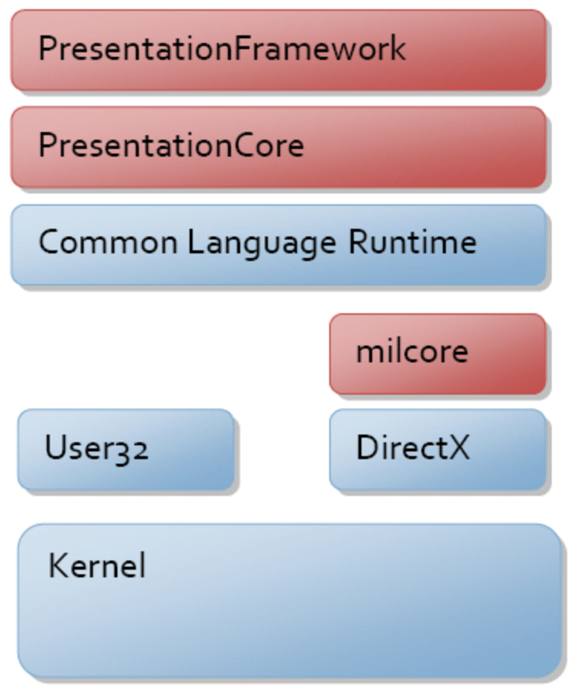
\includegraphics[scale=1]{chapter/uibase/wpf.png}
    \caption{WPF主要组件}
    \label{fig:wpf}
\end{figure}

 WPF的主要组件如图 \ref{fig:wpf} 所示,关系图的红色部分(PresentationFramework、PresentationCore 和 milcore)是 WPF 的主要代码部分。 WPF 中的所有显示都是通过 DirectX 引擎完成的,因此硬件和软件呈现高效。
 
 WPF 作为 .NET 类型的一个子集存在,大部分位于 System.Windows 命名空间中。 
 WPF设计思想是将界面标记描述与实现代码分离,从而实现界面设计(美工)与代码实现(开发人员)并行工作,提升开发效率。
 
界面标记描述使用 XAML,XAML的英文全称为 Extensible Application Markup Language, 翻译为中文为``可扩展应用程序标记语言'',XAML是派生自XML的可扩展应用程序标记语言,以声明形式实现应用程序的外观。 通常用它定义窗口、对话框、页面和用户控件,并填充控件、形状和图形。
  
现代软件开发如Android等,均采用xml等标记语言编写界面,因此WPF的思想以及XAML的方法很值得我们学习。
 
\subsection{WPF核心设计原则}

传统GDI方式与WinForm界面编写方式,均以鼠标拖拽为基础布置界面。

WPF界面设计的核心是:

\begin{enumerate}
    
\item 布局Grid化

摒弃鼠标拖拽这种过于简单方式布局界面,一般的应用将整个Window/Page用Grid进行网格化,再将各个控件按相应的网格行列号布置到相应位置上。

网格宽度与与高度则可设置为自动、指定像素值、按比例设置三种模式,从而控制在界面大小发生改变时,仍然使界面保持合理布局。

\item 数据交换绑定化

传统的界面与数据交换方式是直接向诸如Textbox的Text属性取值,并将其转换为相应数值,提供给相应算法进行计算,再将计算结果赋值到界面元素的相应属性中。

这种方式简单、直接。但在数据的容错处理上十分困难,从而导致程序的健壮性、功能正确性上也受到影响。

WPF为我们提供了数据绑定的方式进行数据交换。

\item 数据驱动界面化

WPF以数据为中心,数据驱动界面,而不是传统的事件驱动。

WPF是通过样式、控件模板、数据模板等方式实现了数据驱动界面。


\end{enumerate}



\section{XAML基本语法}

由于课时与篇幅的原因,此处对WPF的设计原理不做过多的论述,我们直接生成一个实例来分析XAML的语法。

\subsection{WPF项目结构}
我们基于 .net 6 生成一个默认的 WPF 项目,项目结构如图\ref{fig:wpfsln}所示:

\begin{figure}[htbp]
    \centering
    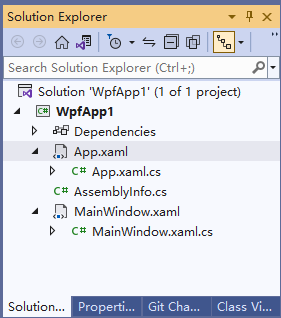
\includegraphics[scale=1]{chapter/uibase/wpfsln.png}
    \caption{WPF项目结构}
    \label{fig:wpfsln}
\end{figure}

项目中主要有两个文件App.xaml 与 MainWindow.xaml。每个xaml文件都有一个相应的扩展名为cs
的后台编码文件。

\subsection{项目中的xaml文件及含义}
App.xaml文件主要描述了项目的初始信息,代码如下:
\begin{lstlisting}[language=xml]
<Application x:Class="WpfApp1.App"
    xmlns="http://schemas.microsoft.com/winfx/2006/xaml/presentation"
    xmlns:x="http://schemas.microsoft.com/winfx/2006/xaml"
    xmlns:local="clr-namespace:WpfApp1"
    StartupUri="MainWindow.xaml">
    <Application.Resources>
    
    </Application.Resources>
</Application>
\end{lstlisting}

最主要的就是StartupUri 属性指定了该Application的启动地址是  "MainWindow.xaml" 文件。

 MainWindow.xaml文件描述了启动的主窗体,代码如下:

 \begin{lstlisting}[language=xml]
<Window x:Class="WpfApp1.MainWindow"
        xmlns="http://schemas.microsoft.com/winfx/2006/xaml/presentation"
        xmlns:x="http://schemas.microsoft.com/winfx/2006/xaml"
        xmlns:d="http://schemas.microsoft.com/expression/blend/2008"
        xmlns:mc="http://schemas.openxmlformats.org/markup-compatibility/2006"
        xmlns:local="clr-namespace:WpfApp1"
        mc:Ignorable="d"
        Title="MainWindow" Height="450" Width="800">
    <Grid>

    </Grid>
</Window>
\end{lstlisting}

文件中出现的 xmlns为文件中引入的命名空间,xmlns 为 xml namespace的缩写。

从这两个文件可以看出,每个xaml文件都是一颗xml的树,这棵树的根为Application、Window、Page等等。







%%%%%%%%%%%%%%%%%%%%%%%%%%%%%%%%%%%%%%
\section{WPF常用控件}

WPF控件基本上可以分为六类:

\begin{enumerate}
    \item 布局控件
    
    可以容纳多个控件或嵌套其它布局控件,用于在UI上组织和排列控件。如Grid、StackPanel、DockPanel等。
    
    \item 内容控件
    
    只能容纳一个其它控件或布局控件作为它的内容。Window、Button等均属于该类,是继承于类ContentControl。
    
    \item 带标题内容控件
    
    相当于一个内容控件,但可以加一个标题(Header),如GroupBox、TabItem等,是继承于类HeaderedContentControl。
    
    \item 条目控件
    
    可以显示一系列的数据,如ListBox、ComboBox等,它们继承于类ItemsControl。
    
    \item 带标题条目控件
    
    相当于一个条目控件加上一个标题显示区,如TreeViewItem、MenuItem等,用于显示层级关系数据,节点显示在Header区域,子节点显示在条目控件区域。它们继承于类HeaderedItemsControl。
    
    \item 特殊内容控件
    
    如TextBox容纳的字符串,TextBlock容纳的可自由控制格式的文本, Image容纳图片类型数据。
    
\end{enumerate}




%%%%%%%%%%%%%%%%%%%%%%%%%%%%%%%%%%%%%%
\section{坐标方位角计算图形界面程序编写}

前面我们编写了坐标方位角计算算法函数与角度弧度互相转换的函数。这节我们将借助于
WPF界面编写技术完成一个较为完整的图形界面的坐标方位角程序的编写。

\subsection{建立解决方案与项目}
启动Visual Studio(本书中所用版本为2017英文版),依次点击菜单File -> New -> Project...,
在弹出的对话框中按图\ref{fig:AzimuthApp1}所示输入新建项目名称、选择项目类型等。

\begin{figure}[htbp]
    \centering
    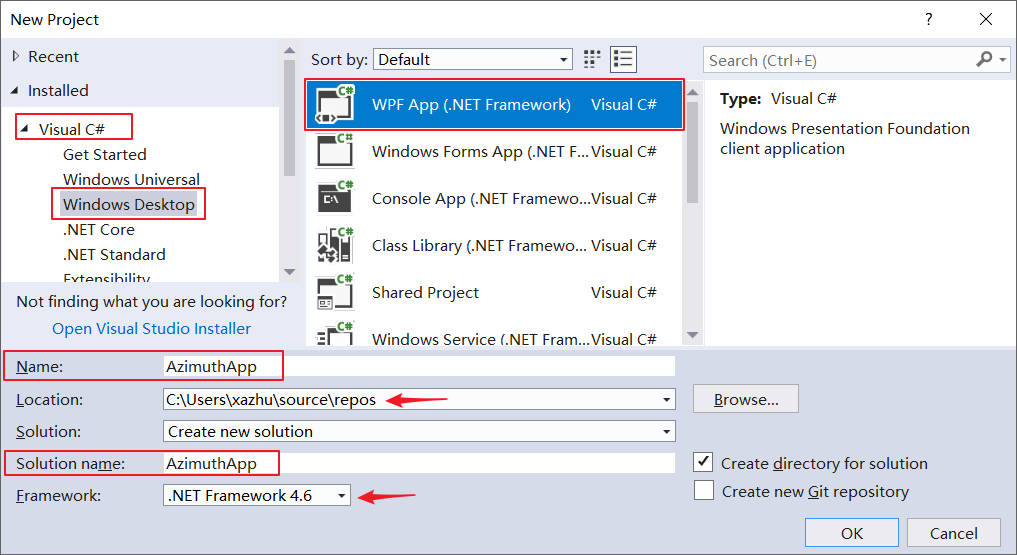
\includegraphics[scale=0.6]{chapter/surveybase/AzimuthApp1.png}
    \caption{新建项目示意图}
    \label{fig:AzimuthApp1}
\end{figure}

建好后的项目如图\ref{fig:AzimuthApp2}所示:

\begin{figure}[htbp]
    \centering
    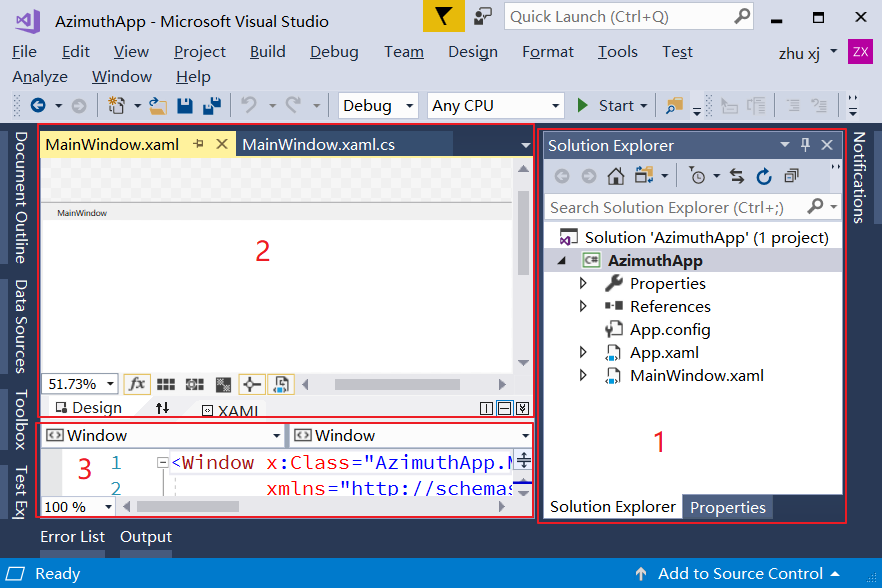
\includegraphics[scale=0.6]{chapter/surveybase/AzimuthApp2.png}
    \caption{方位角计算项目示意图}
    \label{fig:AzimuthApp2}
\end{figure}

由图\ref{fig:AzimuthApp2}可以看出,Visual Studio是以Solution、Project、File
的形式组织管理的。一个Solution可以包括一个至多个Project,一个Project中包含多个文件,
且一个Project编译为一个exe或dll文件,C\#中所有的对象与数据均以文件的形式组织。

图\ref{fig:AzimuthApp2}中的1区为Solution Explorer区,可对Project及File进行各种
操作。2、3区为代码与界面编写区,文件类型不同,呈现的内容也会不一样。

现代软件开发应遵循界面与算法分离的原则,因此我们再新建一类库项目SMath,用于
组织我们的算法,如图\ref{fig:AzimuthApp3}所示:

\begin{figure}[htbp]
    \centering
    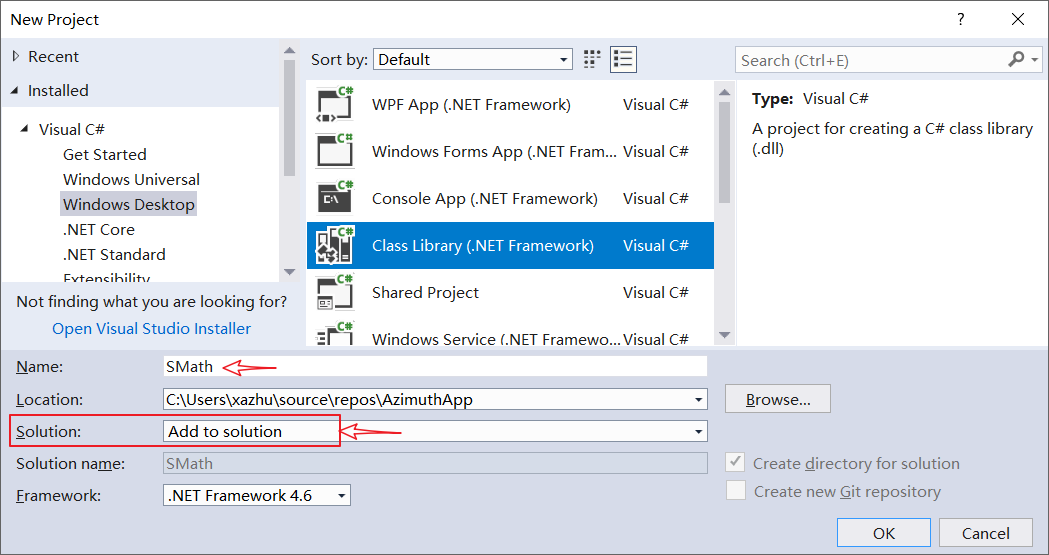
\includegraphics[scale=0.6]{chapter/surveybase/AzimuthApp3.png}
    \caption{新建类库项目示意图}
    \label{fig:AzimuthApp3}
\end{figure}

在该步操作中除了项目类型应选择Class Library之外,与图\ref{fig:AzimuthApp1}
不同的是此处Solution项应选择Add to solution而不是原来的 Create new solution。

现代软件开发的另一个原则是保证代码的可测试性,在增加类库项目后,
再增加一单元测试项目UnitTestSMath。鼠标右击图\ref{fig:AzimuthApp2}中的Solution Explorer区
中的Solution 'AzimuthApp'项,在弹出的右键快捷菜单中选择 Add,
在 Add 的下级菜单中选择 New Project..., 将弹出如图\ref{fig:AzimuthApp6}所示的添加单元测试项目的
对话框。

\begin{figure}[htbp]
    \centering
    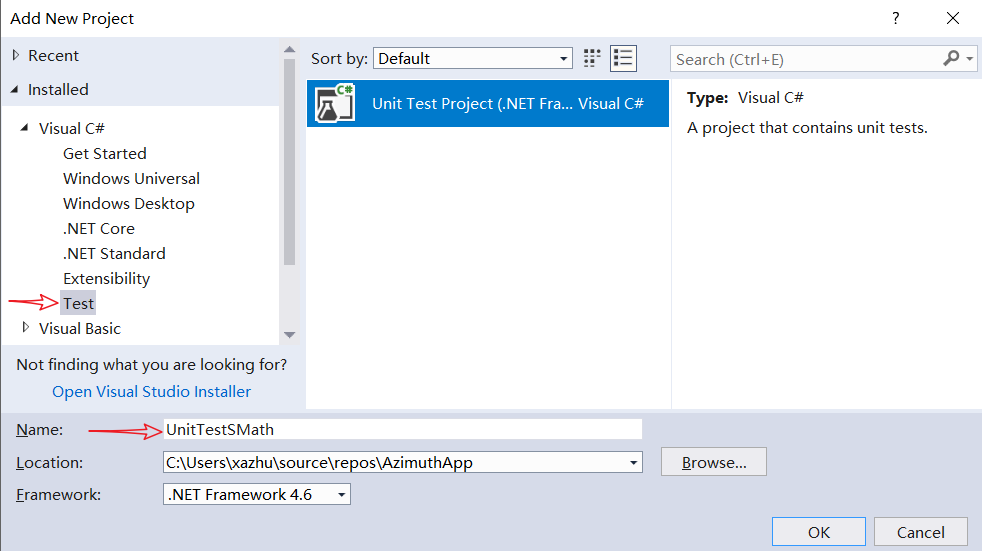
\includegraphics[scale=0.6]{chapter/surveybase/AzimuthApp6.png}
    \caption{添加单元测试项目示意图}
    \label{fig:AzimuthApp6}
\end{figure}

在图\ref{fig:AzimuthApp6}的操作中,应在左侧选择Test,在右边选择 Unit Test Project,

整个操作完成后,我们的解决方案Solution就拥有三个项目了,如图\ref{fig:AzimuthApp7}所示。
项目AzimuthApp为我们的界面编写项目,是启动项目(StartUp Project)。
项目SMath为我们的算法项目,项目UnitTestSMath为
对算法项目SMath进行单元测试的项目。

\begin{figure}[htbp]
\centering
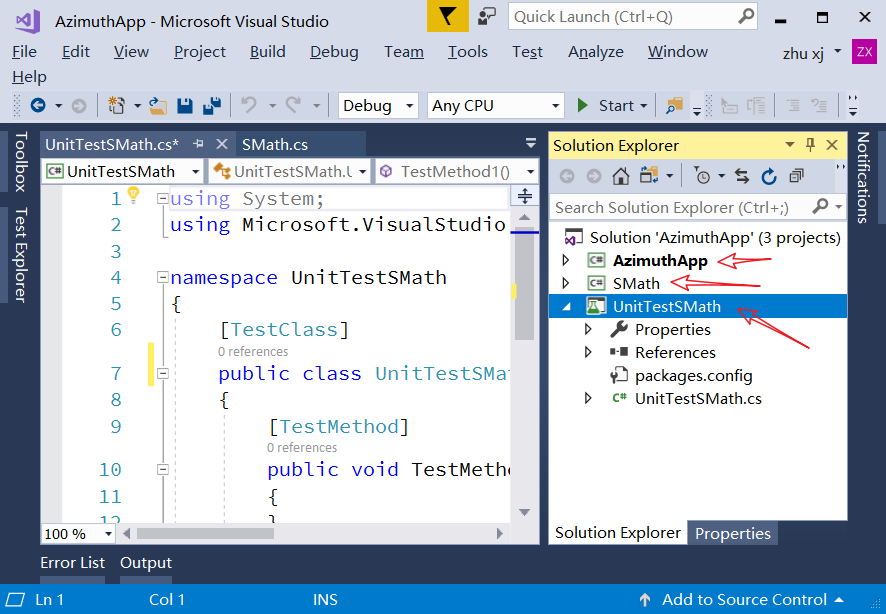
\includegraphics[scale=0.7]{chapter/surveybase/AzimuthApp7.png}
\caption{完整的Solution示意图}
\label{fig:AzimuthApp7}
\end{figure}

下面我们通过添加引用或参考(Add Reference)为三个项目建立关系。

SMath项目为基础算法,AzimuthApp需要用到其中的算法,因此应该向AzimuthApp项目
添加对SMath项目的引用。点击AzimuthApp项目将其展开,鼠标右击项目中的References
项,弹出如图\ref{fig:AzimuthApp4}所示的快捷菜单:

\begin{figure}[htbp]
\centering
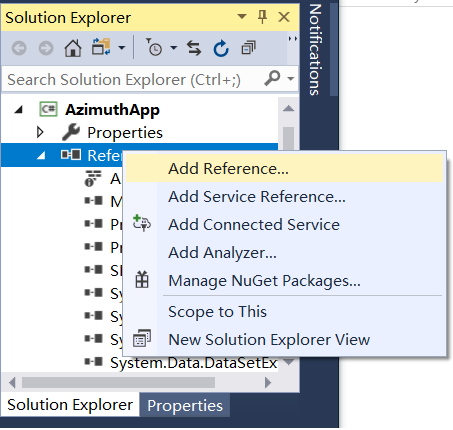
\includegraphics[scale=0.8]{chapter/surveybase/AzimuthApp4.png}
\caption{引用类库项目示意图}
\label{fig:AzimuthApp4}
\end{figure}

点击Add Reference...项,弹出如图\ref{fig:AzimuthApp5}所示的对话框。
在对话框左侧确保选中Projects,在右侧选中SMath项目,单击OK按钮就将引用添加完毕。
同样的方法向UnitTestSMath项目添加对SMath项目的引用。
\begin{figure}[htbp]
\centering
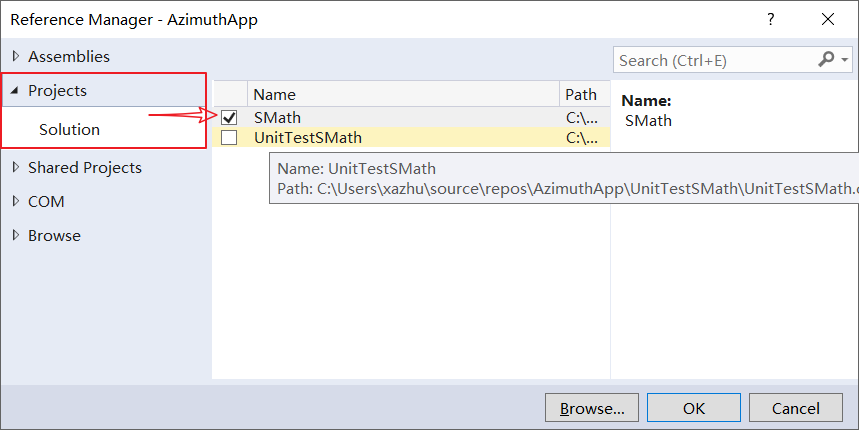
\includegraphics[scale=0.7]{chapter/surveybase/AzimuthApp5.png}
\caption{选择引用类库项目示意图}
\label{fig:AzimuthApp5}
\end{figure}

至此,我们的项目构建完成,整个程序的架构已经搭建好了。
在SMath项目中将原来的Class1.cs文件删除,新添一SMath.cs
文件,在SMath.cs文件中将我们前边讲解的SMath类加入其中,将各个函数组织进来,
对该项目执行构建(build)操作生成Dll类库文件,在另两个项目中就可以使用了。

\subsection{界面编写}

在确保基本算法的正确性后,我们就可以编写界面程序了。我们编写一简单界面,如图\ref{fig:AzimuthUI1}
所示。

\begin{figure}[htbp]
\centering
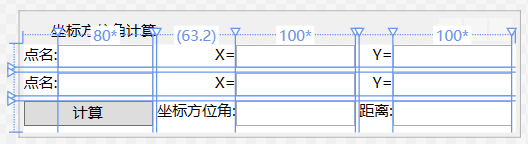
\includegraphics[scale=1]{chapter/surveybase/AzimuthUI1.png}
\caption{坐标方位角计算设计界面}
\label{fig:AzimuthUI1}
\end{figure}

相应的XAML设计代码如下:

\begin{lstlisting}[language=xml]
<Window x:Class="AzimuthApp.MainWindow"
    xmlns="http://schemas.microsoft.com/winfx/2006/xaml/presentation"
    xmlns:x="http://schemas.microsoft.com/winfx/2006/xaml"
    xmlns:d="http://schemas.microsoft.com/expression/blend/2008"
    xmlns:mc="http://schemas.openxmlformats.org/markup-compatibility/2006"
    xmlns:local="clr-namespace:AzimuthApp"
    mc:Ignorable="d"
    Title="坐标方位角计算" Height="100" Width="400">
    <Grid>
        <Grid.ColumnDefinitions>
            <ColumnDefinition Width="Auto"/>
            <ColumnDefinition Width="80*"/>
            <ColumnDefinition Width="3"/>
            <ColumnDefinition Width="Auto"/>
            <ColumnDefinition Width="100*"/>
            <ColumnDefinition Width="3"/>
            <ColumnDefinition Width="Auto"/>
            <ColumnDefinition Width="100*"/>
            <ColumnDefinition Width="3"/>
        </Grid.ColumnDefinitions>
        <Grid.RowDefinitions>
            <RowDefinition Height="Auto"/>
            <RowDefinition Height="3"/>
            <RowDefinition Height="Auto"/>
            <RowDefinition Height="3"/>
            <RowDefinition Height="Auto"/>
        </Grid.RowDefinitions>
        <TextBlock Text="点名:" Grid.Row="0" Grid.Column="0" />
        <TextBox x:Name="textBoxAName" Grid.Row="0" Grid.Column="1" />
        <TextBlock Text="X=" TextAlignment="Right" Grid.Row="0" Grid.Column="3"/>
        <TextBox x:Name="textBoxAX" Grid.Row="0" Grid.Column="4"/>
        <TextBlock Text="Y=" TextAlignment="Right" Grid.Row="0" Grid.Column="6"/>
        <TextBox x:Name="textBoxAY" Grid.Row="0" Grid.Column="7" />
        
        <TextBlock Text="点名:" Grid.Row="2" Grid.Column="0" />
        <TextBox x:Name="textBoxBName" Grid.Row="2" Grid.Column="1" />
        <TextBlock Text="X=" TextAlignment="Right" Grid.Row="2" Grid.Column="3"/>
        <TextBox x:Name="textBoxBX" Grid.Row="2" Grid.Column="4" />
        <TextBlock Text="Y=" TextAlignment="Right" Grid.Row="2" Grid.Column="6"/>
        <TextBox x:Name="textBoxBY" Grid.Row="2" Grid.Column="7" />
        
        <Button x:Name="buttonAzimuth" Content="计算" Grid.Row="5" 
            Grid.Column="0" Grid.ColumnSpan="2" Click="buttonAzimuth_Click"/>
        <TextBlock x:Name="textBlockAzimuth" 
            Text="坐标方位角:" TextAlignment="Right" Grid.Row="5" Grid.Column="3"/>
        <TextBox x:Name="textBoxAzimuth" Grid.Row="5" Grid.Column="4" />
        <TextBlock Text="距离:" TextAlignment="Right" Grid.Row="5" Grid.Column="6" />
        <TextBox x:Name="textBoxDistance" Grid.Row="5" Grid.Column="7" />
    </Grid>
</Window>
\end{lstlisting}

计算按钮的Click事件代码如下:
\begin{lstlisting}
private void buttonAzimuth_Click(object sender, RoutedEventArgs e)
{
    double.TryParse(textBoxAX.Text, out double xA);
    double.TryParse(textBoxAY.Text, out double yA);
    double.TryParse(textBoxBX.Text, out double xB);
    double.TryParse(textBoxBY.Text, out double yB);

    double distanceAB = ZXY.SMath.Azimuth(xA, yA, xB, yB, out double azimuthAB);

    textBoxAzimuth.Text = ZXY.SMath.RADtoString(azimuthAB);
    textBoxDistance.Text = distanceAB.ToString();
    textBlockAzimuth.Text = $"{textBoxAName.Text}->{textBoxBName.Text}坐标方位角:";
}
\end{lstlisting}

程序的运行结果如图\ref{fig:AzimuthUI2}所示。

\begin{figure}[htbp]
    \centering
    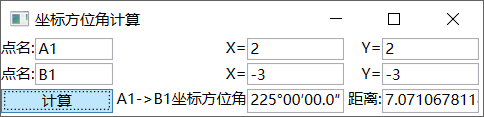
\includegraphics[scale=1]{chapter/surveybase/AzimuthUI2.png}
    \caption{坐标方位角计算运行界面}
    \label{fig:AzimuthUI2}
\end{figure}

\subsection{界面程序的优化}

WPF技术的核心是绑定(Binding),以上程序虽然简单,但也涉及数据与界面的交互问题。
我们对其界面稍加抽象,改写一下。

我们新建一个类AzimuthUI,其代码如下:
\begin{lstlisting}
using System.ComponentModel;

namespace AzimuthApp
{
    class AzimuthUI : INotifyPropertyChanged
    {
        public event PropertyChangedEventHandler PropertyChanged;
        public void RaisePropertyChanged(string propertyName)
        {
            if (PropertyChanged != null)
            {
                PropertyChanged.Invoke(this, new PropertyChangedEventArgs(propertyName));
            }
        }
        
        private string _AName = "";
        public string AName
        {
            get => _AName;
            set
            {
                _AName = value;
                RaisePropertyChanged("AName");
            }
        }
        
        private double _xA;
        public double XA
        {
            get => _xA;
            set
            {
                _xA = value;
                RaisePropertyChanged("XA");
            }
        }
        
        
        private double _yA;
        public double YA
        {
            get => _yA;
            set
            {
                _yA = value;
                RaisePropertyChanged("YA");
            }
        }
        
        private string _BName = "";
        public string BName
        {
            get => _BName;
            set
            {
                _BName = value;
                RaisePropertyChanged("BName");
            }
        }
        
        private double _xB;
        public double XB
        {
            get => _xB;
            set
            {
                _xB = value;
                RaisePropertyChanged("XB");
            }
        }
        
        private double _yB;
        public double YB
        {
            get => _yB;
            set
            {
                _yB = value;
                RaisePropertyChanged("YB");
            }
        }
        
        public string AzimuthName
        {
            get => $"{AName}->{BName}坐标方位角:";
        }
        
        private double _azimuthAB;
        public string AzimuthAB
        {
            get => ZXY.SMath.RADtoString(_azimuthAB);
        }
        
        private double _distanceAB;
        public double DistanceAB
        {
            get => _distanceAB;
        }
        
        public void CalAzimuthDistanceAB()
        {
            _distanceAB = ZXY.SMath.Azimuth(XA, YA, XB, YB, out _azimuthAB);
            RaisePropertyChanged("AzimuthAB");
            RaisePropertyChanged("DistanceAB");
            RaisePropertyChanged("AzimuthName");
        }
    }
}
\end{lstlisting}

界面代码做如下修改:
\begin{lstlisting}[language=XML]
    <TextBlock Text="点名:" Grid.Row="0" Grid.Column="0" />
    <TextBox x:Name="textBoxAName" Text="{Binding AName}" 
    Grid.Row="0" Grid.Column="1" />
    <TextBlock Text="X=" TextAlignment="Right"
    Grid.Row="0" Grid.Column="3"/>
    <TextBox x:Name="textBoxAX" Text="{Binding XA}" 
    Grid.Row="0" Grid.Column="4"/>
    <TextBlock Text="Y=" TextAlignment="Right" 
    Grid.Row="0" Grid.Column="6"/>
    <TextBox x:Name="textBoxAY" Text="{Binding YA}" 
    Grid.Row="0" Grid.Column="7" />
    
    <TextBlock Text="点名:" Grid.Row="2" Grid.Column="0" />
    <TextBox x:Name="textBoxBName" Text="{Binding BName}" 
    Grid.Row="2" Grid.Column="1" />
    <TextBlock Text="X=" TextAlignment="Right" Grid.Row="2" Grid.Column="3"/>
    <TextBox x:Name="textBoxBX" Text="{Binding XB}" 
    Grid.Row="2" Grid.Column="4" />
    <TextBlock Text="Y=" TextAlignment="Right" Grid.Row="2" Grid.Column="6"/>
    <TextBox x:Name="textBoxBY"  Text="{Binding YB}" 
    Grid.Row="2" Grid.Column="7" />
    
    <Button x:Name="buttonAzimuth" Content="计算" Grid.Row="5" 
    Grid.Column="0" Grid.ColumnSpan="2"
    Click="buttonAzimuth_Click"/>
    <TextBlock x:Name="textBlockAzimuth" 
    Text="{Binding AzimuthName, Mode=OneWay}" 
    TextAlignment="Right" Grid.Row="5" Grid.Column="3"/>
    <TextBox x:Name="textBoxAzimuth" Text="{Binding AzimuthAB, Mode=OneWay}" 
    Grid.Row="5" Grid.Column="4" />
    <TextBlock Text="距离:" TextAlignment="Right" Grid.Row="5" Grid.Column="6" />
    <TextBox x:Name="textBoxDistance" Text="{Binding DistanceAB, Mode=OneWay}"
    Grid.Row="5" Grid.Column="7" />
\end{lstlisting}

MainWindow窗体的后代代码做如下修改:

\begin{lstlisting}
namespace AzimuthApp
{
    public partial class MainWindow : Window
    {
        AzimuthUI azimuthUI;
        public MainWindow()
        {
            InitializeComponent();
            
            azimuthUI = new AzimuthUI();
            this.DataContext = azimuthUI;
        }
        
        private void buttonAzimuth_Click(object sender, RoutedEventArgs e)
        {
            azimuthUI.CalAzimuthDistanceAB();
        }
    }
}
\end{lstlisting}